\documentclass[11pt, oneside]{article}   	% use "amsart" instead of "article" for AMSLaTeX format
\usepackage{geometry}                		% See geometry.pdf to learn the layout options. There are lots.
\geometry{letterpaper}                   		% ... or a4paper or a5paper or ... 
%\geometry{landscape}                		% Activate for for rotated page geometry
%\usepackage[parfill]{parskip}    		% Activate to begin paragraphs with an empty line rather than an indent
\usepackage{graphicx}				% Use pdf, png, jpg, or eps� with pdflatex; use eps in DVI mode
								% TeX will automatically convert eps --> pdf in pdflatex		
\usepackage{amssymb}
\usepackage{amsmath}
\usepackage{parskip}

\graphicspath{{/Users/telliott_admin/Dropbox/Tex/png/}}

\title{Feynman and Kepler}
\date{}
\begin{document}
\maketitle
\Large

I am trying to set out the arguments made by Feynman with respect to Kepler's laws, starting with the form in the book \emph{Feynman's Lost Lecture}.

Here is a sketch of an ellipse

\begin{center} 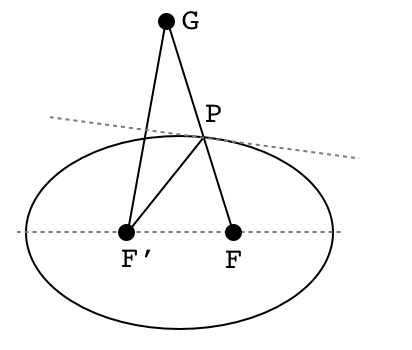
\includegraphics [scale=0.6] {kepler1.png} \end{center}

We pick a point $P$ on the graph of the ellipse and draw the tangent to the curve at that point (if it doesn't look perfect, that may be due to the fact that I just estimated the positions of the foci $F$ and $F'$).  Now construct $F'G$ such that it is perpendicular to the tangent line.  Draw $GP$.  

The two triangles formed by this construction within $\triangle F'GP$ are congruent.  In particular, $F'P$ is equal to $GP$, and the angle $GP$ makes with the tangent line is equal to the angle $F'P$ makes with the tangent line.

Our intermediate goal is to prove that $FPG$ is a straight line.  If this is true then we will have proven that the angle that $FP$ makes with the tangent line will be equal to the angle that $F'P$ makes with the tangent line.

Now, point $P$ is on the tangent line and also on the ellipse, at the point where they touch.  No other point on the tangent line is closer to the foci.

\begin{center} 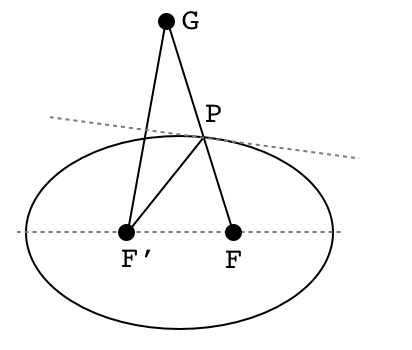
\includegraphics [scale=0.6] {kepler1.png} \end{center}

To see this, pick another point that is on the tangent line (and outside the ellipse), and is also supposedly closer, $Q$.  But the sum of the distances $FQ + F'Q$ will be greater than for $FP + F'P$ because, $Q$ is \emph{outside the ellipse}.

Since choice of $P$ at the point of tangency minimizes the distance $FP + F'P$ and since $F'P = GP$, $P$ also minimizes the distance $FP + GP$.  Therefore, $FG$ is a straight line.  That's the argument for part one.





\end{document}  